% !TEX root = ../../main.tex
\section{One-Class Classification}\label{sec:one_class_classification}

*** TODO: bridge that explains why \gls{occ} is interesting ***

\subsection{Problem formulation}\label{subsec:occ-problem-formulation}
*** Introduce problem of \gls{occ}. Relate to two-class classification. ***

The problem of \gls{occ} is closely related to the (traditional) two-class classification situation\footnote{Two-class problems are considered as to be the basic problem, since multi-class classification problems can be decomposed into multiple two-class problems \cite{fukunaga1990introduction}.}.
In the case of traditional classification algorithms, the problem is to classify an unknown object to one of the pre-defined categories.
This problem is solved by determining a decision boundary in the feature space of the data objects and label the new data object based on the location relative to this boundary.



In case of the \gls{occ} problem, only one class (often refered to as the target class) of data is available in the training phase, or the aquisition of outliers is very expensive.

Figure \ref{fig:two-vs-one-classification} graphically shows the difference between two and one-class classification and the consequences for outlier objects.

\begin{figure}
  \centering
    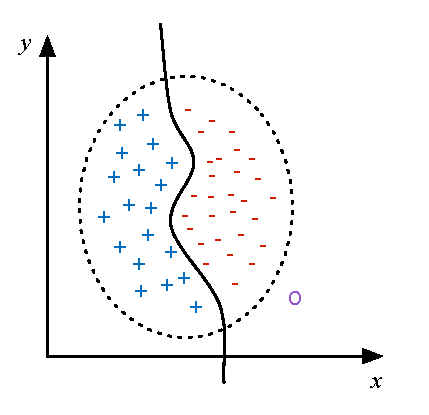
\includegraphics[width=0.5\textwidth,keepaspectratio]{./Figures/chapter3/two-vs-one-classification.pdf}
  \caption[Difference between two and one-class classification]{This plot shows the difference between two and one-class classification. The solid line indicates a possible decision boundary between the $+$ and $*$ example objects. The dashed circle indicates the closed boundary around all the data objects. In the first type the object $o$ is considered to be member of the $*$-class, whilst in the latter (\gls{occ}) formulation it is an outlier.}
  \label{fig:two-vs-one-classification}
\end{figure}



\subsection{One-Class Classification methods}\label{subsec:occ-methods}
In his thesis \cite{tax2001one}, Tax orders a collection of \gls{occ}-methods into three categories, visually represented in Figure \ref{fig:occ-methods}.
The first category consists of methods that estimate the density of the training data and set a threshold on this density.
Among those are Gaussian models, \glspl{gmm} and Parzen density estimators.
In order to get good generalization results with these methods, the dimensionality of the data and the complexity of the density need to be restricted.
This can cause a large bias on the data.
When a good probability model is assumed, these methods work very well, since when one threshold is optimized, a minimum volume is automatically found for the given probability density model \cite{tax2001one}.

Boundary methods are based on Vapnik's principle\footnote{With a limited amount of data available, on should avoid solving a more general problem as an intermediate step to solve the original problem \cite{vapnik1998statistical}.} which imply in this case that estimating the complete data density for a \gls{occ} may be too complex, in case one is only interested in the closed boundary.
Examples of methods that focus on the boundary (a direct threshold) of the training data distribution are K-centers, Nearest-neighborhood and \gls{svdd}.
Especially the latter has a strong bias towards minimal volume solutions.
These type of methods are sensitive to scaling of features, since they rely on a well-defined distance measure.
The number of objects that is required is smaller then in the case of density methods.
The boundary method \gls{svdd}, constructed by Tax, will be further discussed in Section \ref{subsec:oc-svm-svdd}.

Reconstruction methods take a different approach.
Instead of focusing on classification of the data and thus on the discriminating features of data objects, they model the data.
This results in a compact representation of the target data and for any object a reconstruction error can be defined.
Outliers are data objects with a high reconstruction error, since they are worse represented by the constructed model.
Examples of reconstruction methods are K-means, \gls{pca} and some neural network implementations.

\begin{figure}
  \centering
    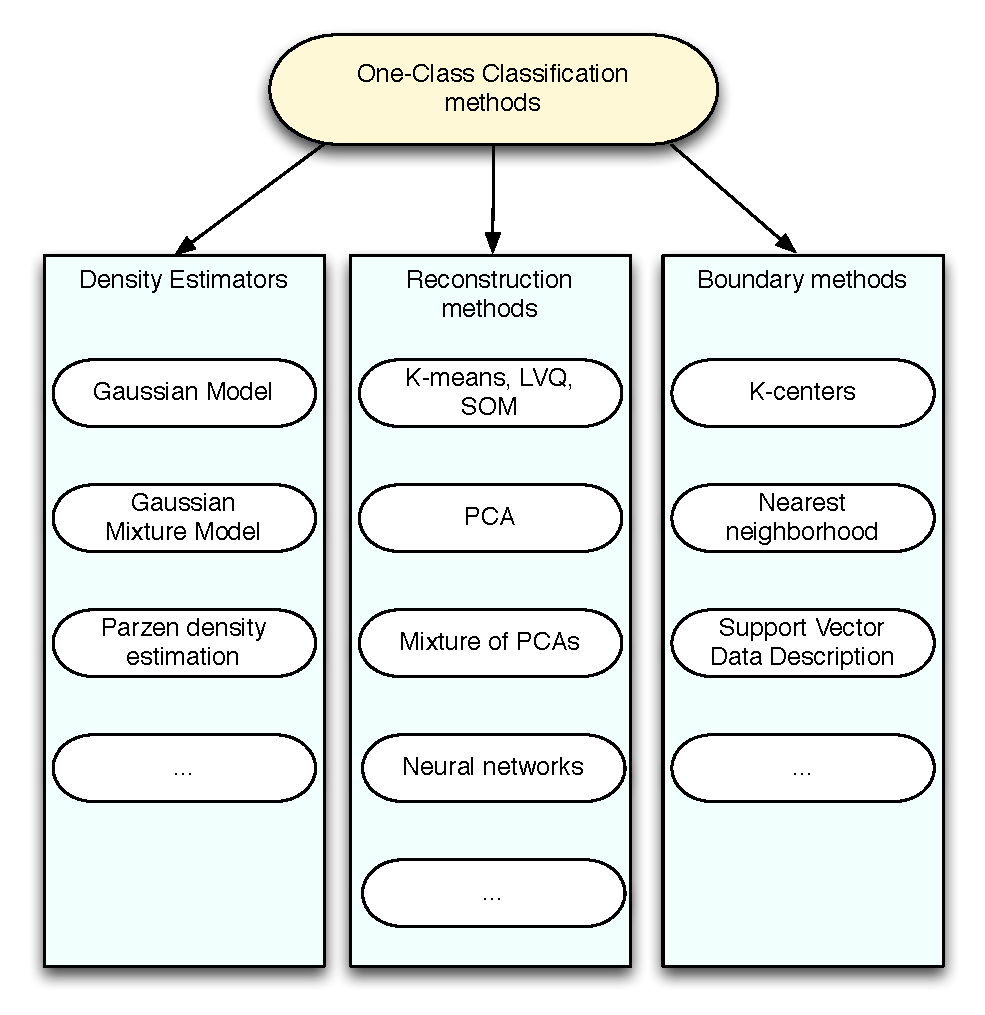
\includegraphics[width=0.5\textwidth,keepaspectratio]{./Figures/chapter3/occ_methods.pdf}
  \caption[\gls{occ} methods]{Overview of \gls{occ} methods categorized in Density Estimators, Reconstruction methods and Boundary methods. This categorization follows the definition of Tax in \cite{tax2001one}.}
  \label{fig:occ-methods}
\end{figure}

*** TODO: end with bridge to next chapter, \gls{oc-svm} ***

-- Literature --

``A survey of recent trends in one class classification'' \cite{khan2010survey}. 25, 2010 \\

``One-class classification by combining density and class probability estimation'' \cite{hempstalk2008one}. 51, 2008 \\

``On simple one-class classification methods'' \cite{noumir2012simple}. 2012 \\

``One-class classification'' \cite{tax2001one}. 693, 2001 \\

``The One-Class Classification Approach to Data Description and to Models Applicability Domain'' \cite{baskin2010one}. 19, 2009 \\

``One-class classifier networks for target recognition applications'' \cite{moya1993one}. 70, 1993. Origin of term ``One-Class Classification'' \\